\documentclass{article}

\usepackage[utf8]{inputenc}
\usepackage{enumitem}
\usepackage{float}
\usepackage{circuitikz}
\usepackage{todonotes}
\usepackage{amsmath}
\usepackage{tikz}
\usetikzlibrary{shapes, calc, shapes, arrows}

\title{Blatt 3}
\author{Luca Krüger, Jonas Otto, Jonas Merkle (Gruppe R)}
\date{\today}

\begin{document}
\maketitle

\section{Lernregeln}
$$E(w,b)=\frac{1}{2}\sum_{\mu=1}^{M}(T_{\mu}-f(wx_{\mu}+b))^2$$
\begin{enumerate}
  \item
        \begin{align*}
          \nabla E(w,b)=\begin{pmatrix} \dfrac{\strut \partial E}{\strut \partial w} \\ \dfrac{\strut \partial E}{\strut \partial b}\end{pmatrix} = \begin{pmatrix}
            - \sum_{\mu=1}^{M}(T_{\mu}-f(wx_{\mu}+b)) \cdot f'(wx_{\mu}+b)\cdot x_{\mu} \\
            - \sum_{\mu=1}^{M}(T_{\mu}-f(wx_{\mu}+b)) \cdot f'(wx_{\mu}+b)
          \end{pmatrix} \\
        \end{align*}
  \item
        \todo[inline]{Lernrate $\eta$}
        \begin{enumerate}[label=\alph*)]
          \item inkrementelle Version:
                \todo[inline]{Woher kommt der Faktor $\mu$?}
                \begin{align*}
                  w(t+1) & =w(t)-\mu(T_{t}-f(wx_{t}+b)) \cdot \dfrac{\strut \partial f(wx_{t}+b)}{\strut \partial w}\cdot x_t \\
                  b(t+1) & =b(t)-\mu(T_{t}-f(wx_{t}+b)) \cdot \dfrac{\strut \partial f(wx_{t}+b)}{\strut \partial w}
                \end{align*}
          \item Batch Version:
                \begin{align*}
                  w(t+1) & =w(t)+\mu\sum_{\mu=1}^{M}(T_{\mu}-f(wx_{\mu}+b)) \cdot \dfrac{\strut \partial f(wx_{\mu}+b)}{\strut \partial w}\cdot x_{\mu} \\
                  b(t+1) & =b(t)+\sum_{\mu=1}^{M}(T_{\mu}-f(wx_{\mu}+b)) \cdot \dfrac{\strut \partial f(wx_{\mu}+b)}{\strut \partial w}                 \\
                         & \text{mit}\ \mu \approx 1/M
                \end{align*}
        \end{enumerate}
  \item
        \begin{enumerate}[label=\alph*)]
          \item \todo[inline]{Python verlinken??}
          \item \todo[inline]{Mathematica Grafik mit Startwerten einfügen}
                \begin{figure}[H]
                  % body of the figure
                  \centering
                  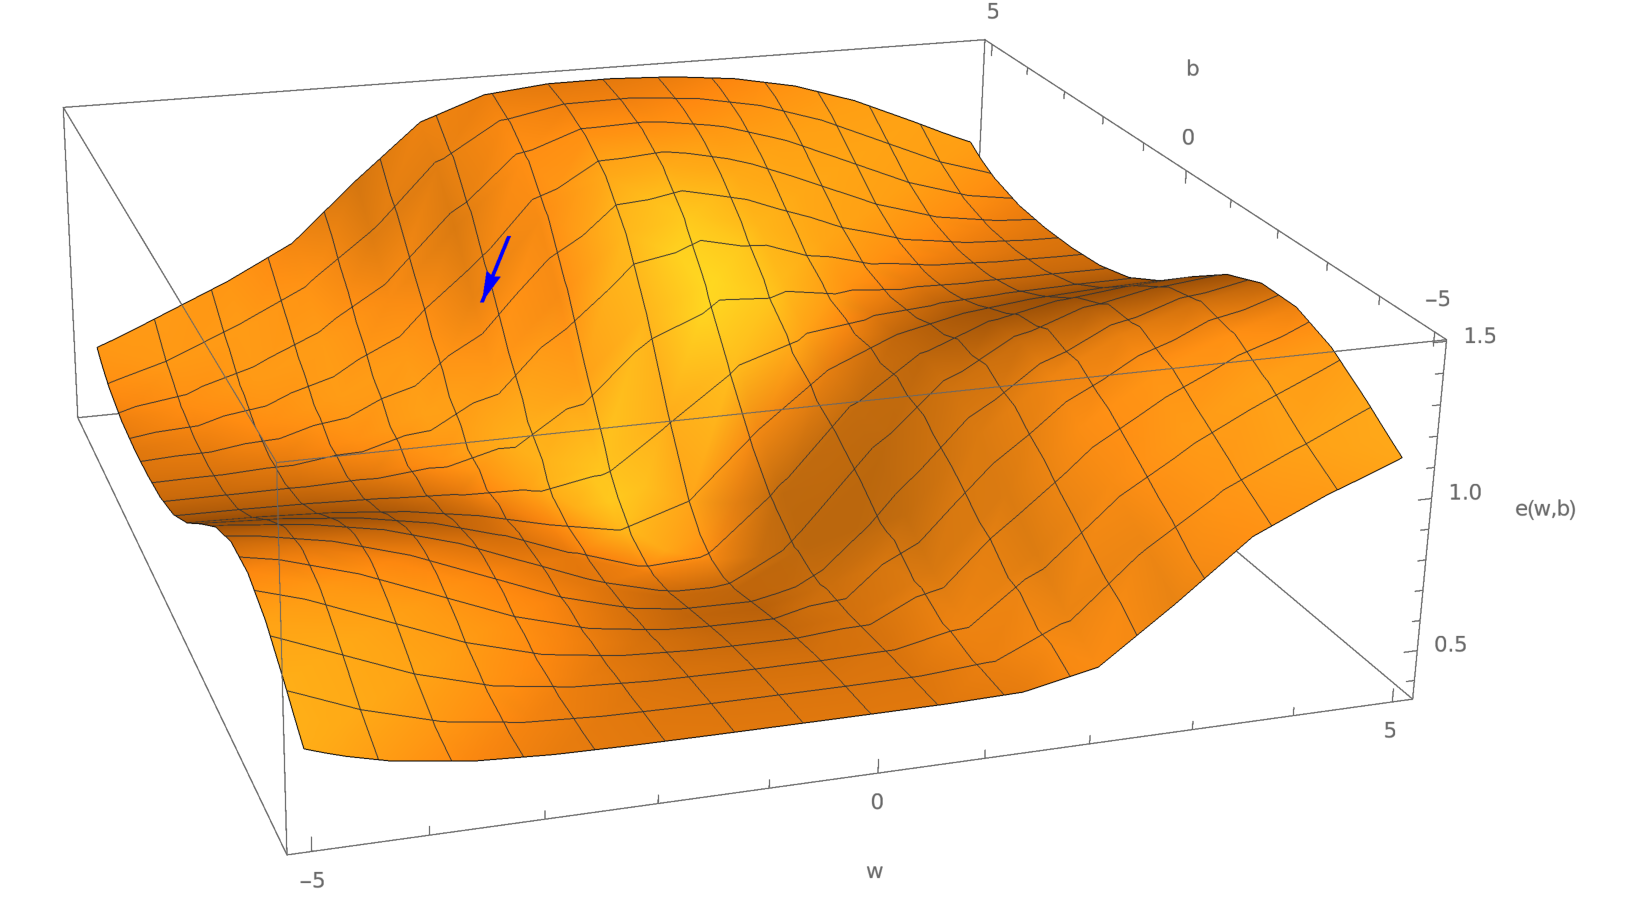
\includegraphics{initial-error-gradient.pdf}
                  \caption{Gradient bei $t=0$}
                \end{figure}

          \item
          \item Der Pfad in Abbildung 3 auf dem Übungsblatt verläuft vom Startpunkt in ein lokales Minimum der Errorfunktion mit hohen Werten für $w$ und $b$.  Problematisch an der Gradienten-Lernregel $E(t)$ ist, dass im allgemeinen gilt $E(t_1)>E(t_2)$ für zwei aufeinanderfolgende Lernschritte $t_1, t_2$ und somit ein Minimum nur in einer lokal monoton fallenden Umgebung des Startpunktes gefunden werden kann. D.h., der Endpunkt des Pfades hängt bei der Lernregel stark von den Anfangswerten ab und ein gefundendes Minimum ist nicht zwangsweise ein globales Minimum der Errorfunktion.
        \end{enumerate}
  \item
        \begin{enumerate}[label=\alph*)]
          \item Pfad 1 wurde mit der
          \item
        \end{enumerate}
\end{enumerate}



\end{document}
